% !TEX encoding = UTF-8
% !TEX TS-program = pdflatex
% !TEX root = ../tesi.tex

\chapter{Fast-Broadcast modifications}
	\label{chapter:fbmod}
	The previous work \cite{ROM2017} utilized a version of Fast-Broadcast in which vehicles having origin-vehicle distance smaller than origin-sender distance suppressed their scheduled transmission since they do not contribute in the outward propagation of the message. In the following graphs, the old version will be called \textit{TD-Fast-Broadcast} (as in \textit{Triangular-Distance-Fast-Broadcast}). The aim of this appendix is to show the reasons why this additional check has been removed in the version of the Fast-Broadcast algorithm used in this work thanks to simulations which employed two scenarios. More in detail, the aim of these simulations has been twofold:
	\begin{itemize}
		\item show that TD-Fast-Broadcast performs worse than Fast-Broadcast in terms of delivery ratios in difficult scenarios with buildings, particularly the Padua urban scenario;
		\item show that Fast-Broadcast is non-pejorative in all metrics in scenarios where TD-Fast-Broadcast did not show delivery ratio problems, such as the Los Angeles urban scenario.
	\end{itemize}

	\section{Fast-Broadcast's improvement on delivery ratios}
		\begin{figure}[H]
			\centering
			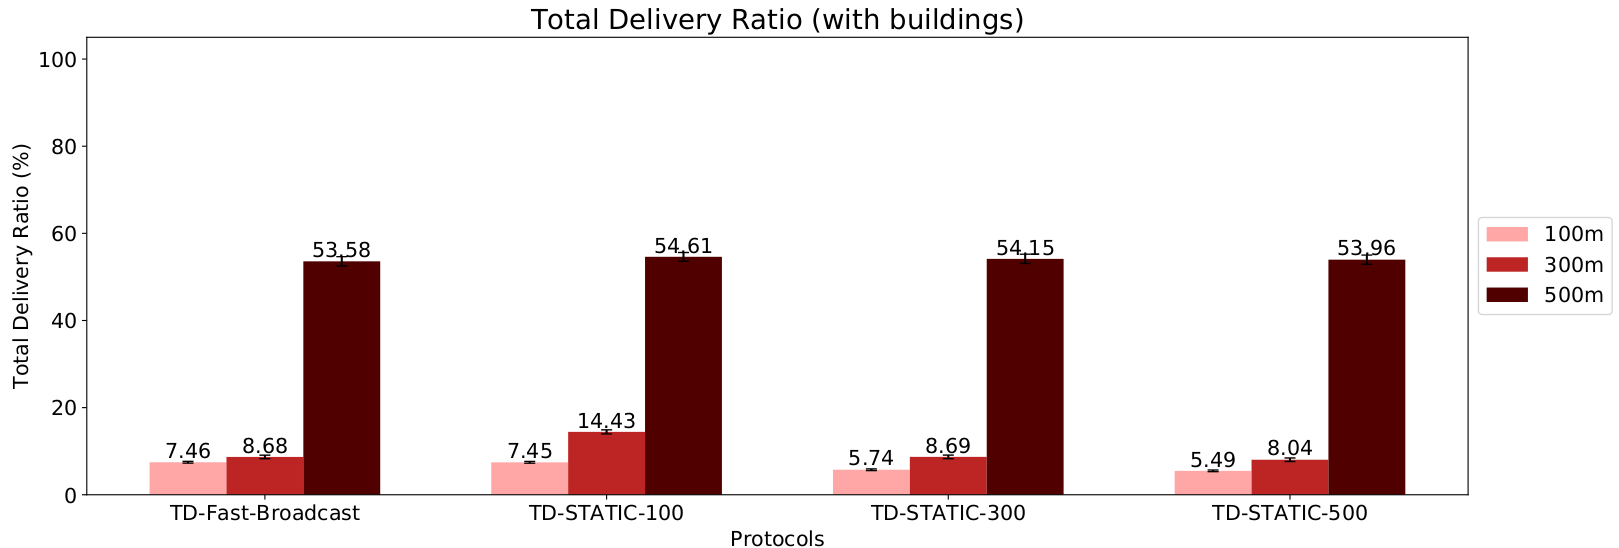
\includegraphics[width=1.0\textwidth]{immagini/td-fb-pd/td-fb/tdr}
			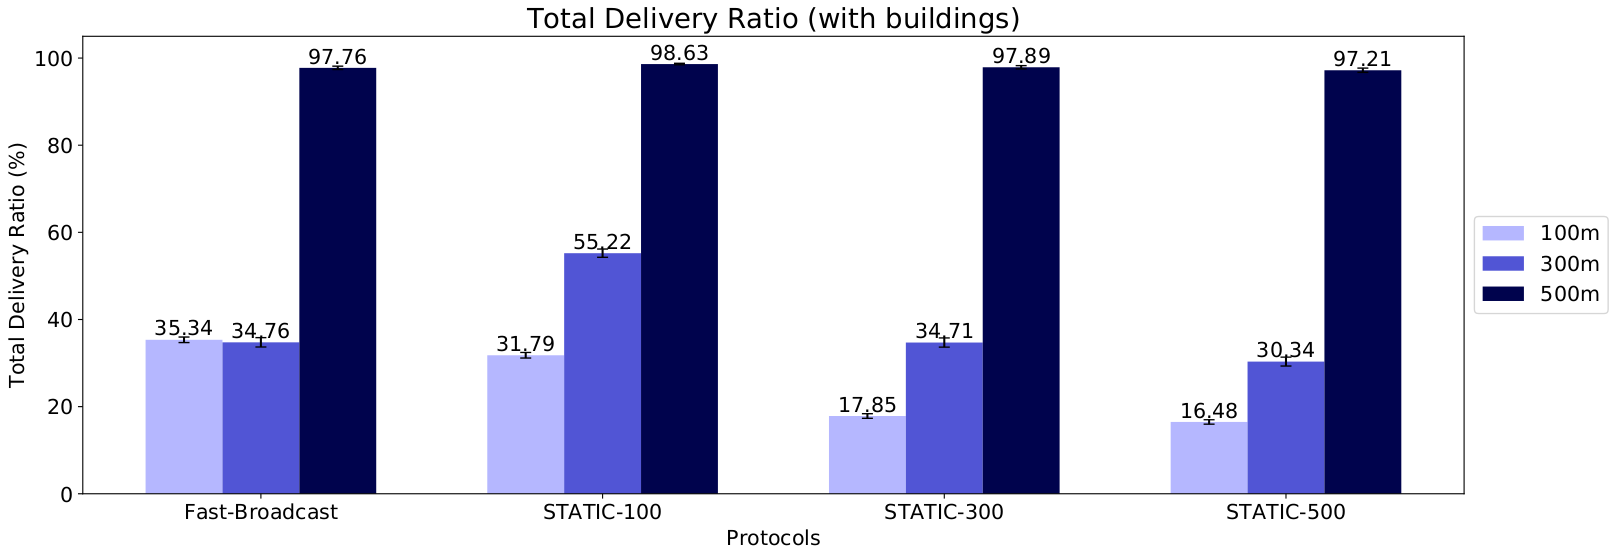
\includegraphics[width=1.0\textwidth]{immagini/td-fb-pd/fb/tdr}
			\caption{\textit{TDR} for TD-Fast-Broadcast (top) and Fast-Broadcast (bottom) for Padua urban scenario}
			\label{fig:td-tdr}
		\end{figure}
	
		\begin{figure}[H]
			\centering
			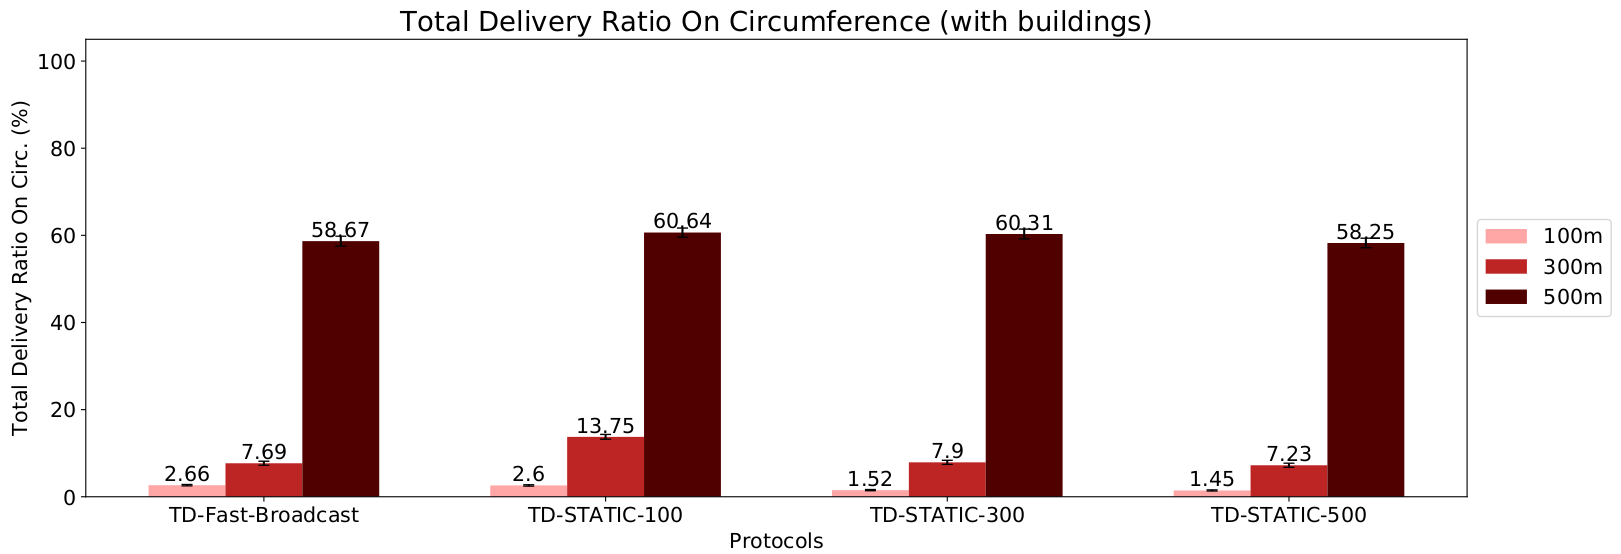
\includegraphics[width=1.0\textwidth]{immagini/td-fb-pd/td-fb/tdroc}	
			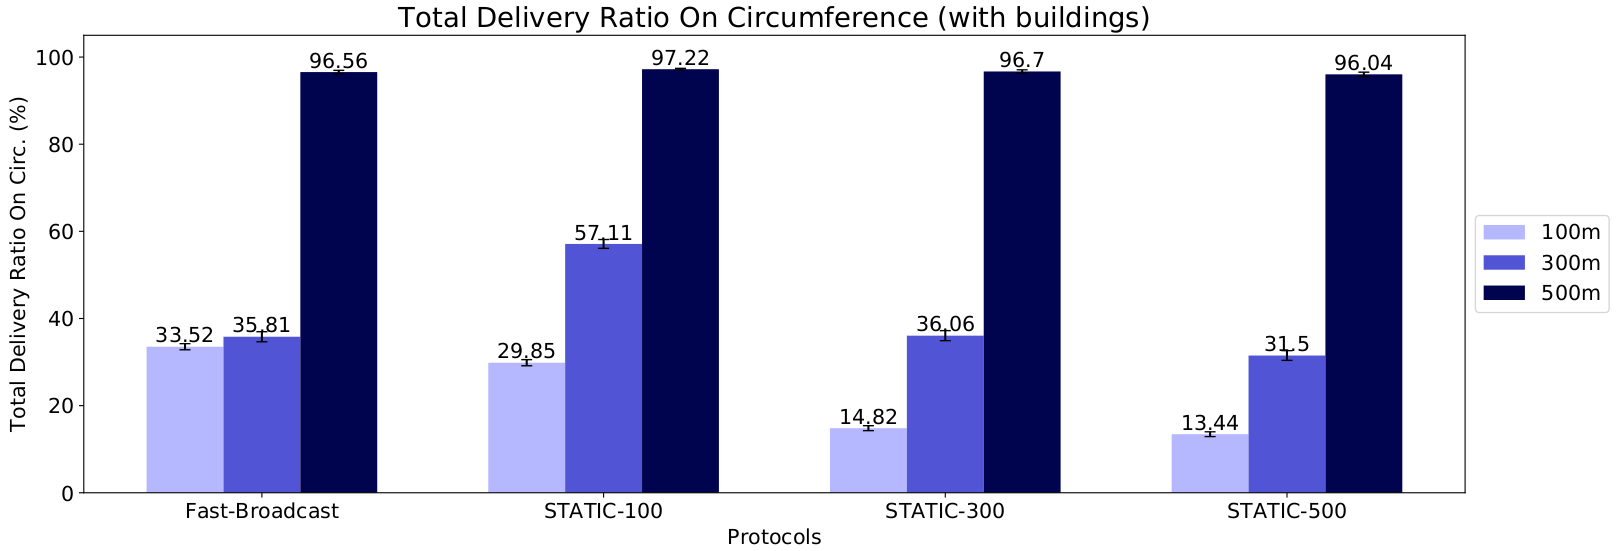
\includegraphics[width=1.0\textwidth]{immagini/td-fb-pd/fb/tdroc}
			\caption{\textit{TDROC} for TD-Fast-Broadcast (top) and Fast-Broadcast (bottom) for Padua urban scenario}
			\label{fig:td-tdroc}
		\end{figure}
	
		\begin{figure}[H]
			\centering
			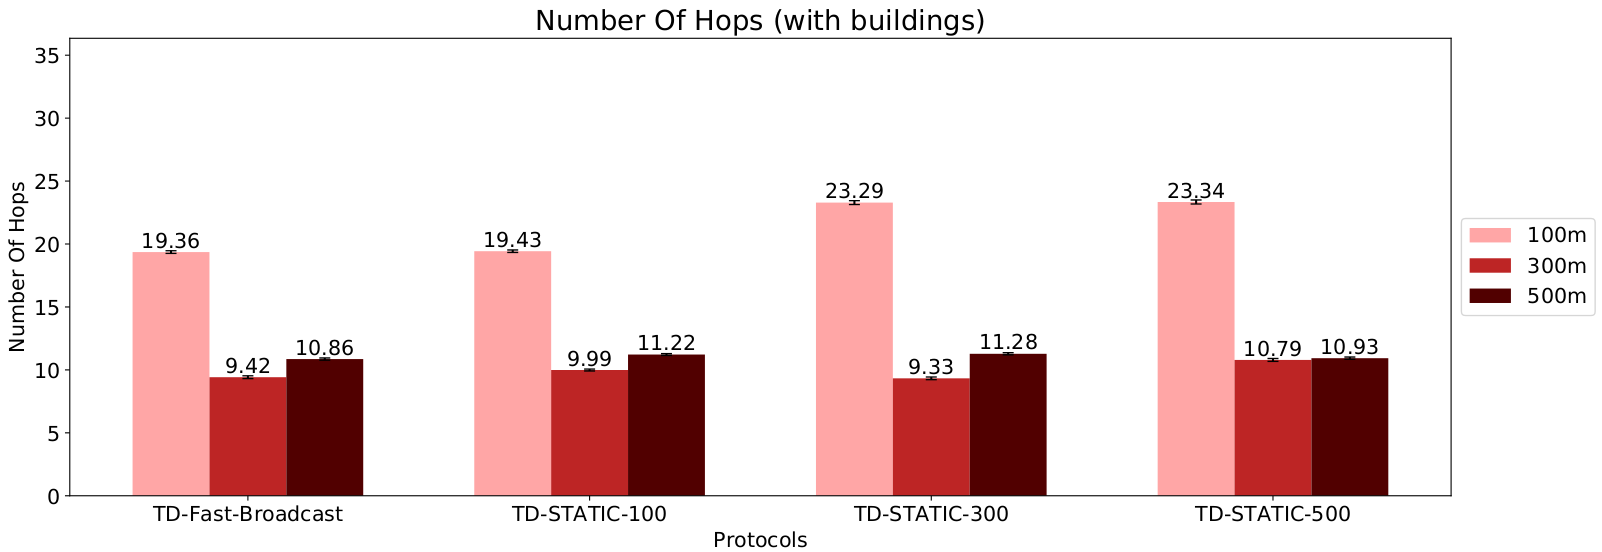
\includegraphics[width=1.0\textwidth]{immagini/td-fb-pd/td-fb/noh}	
			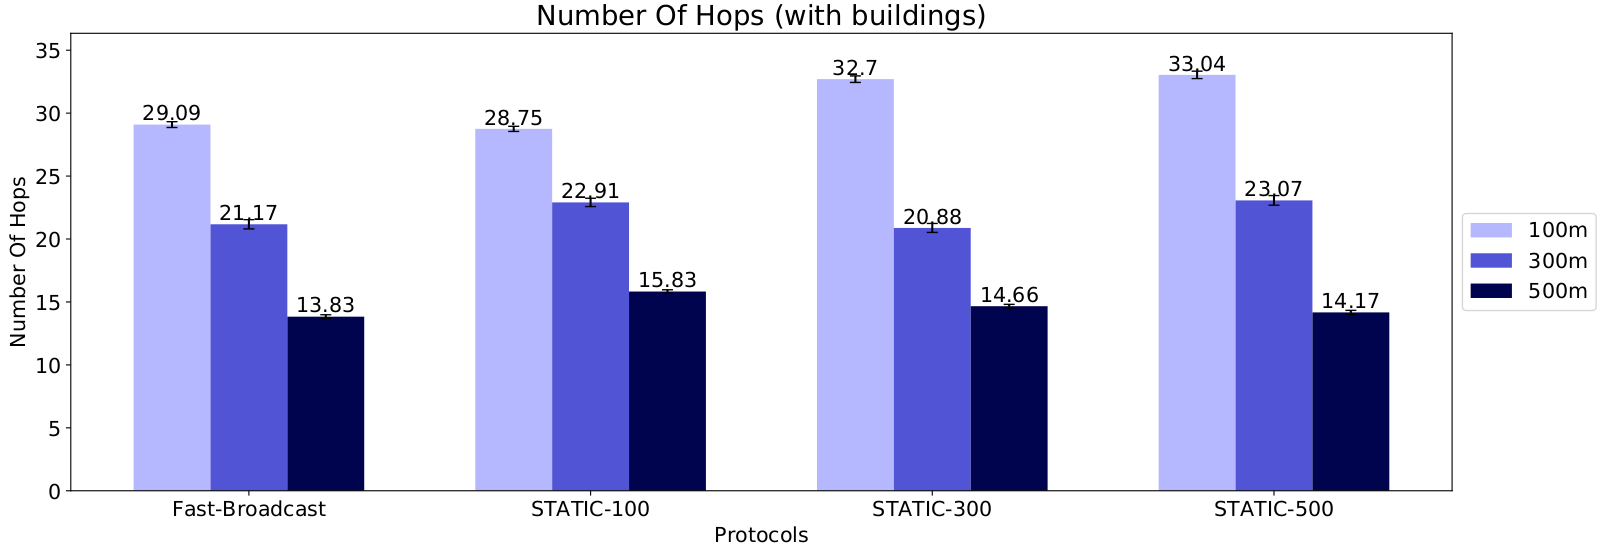
\includegraphics[width=1.0\textwidth]{immagini/td-fb-pd/fb/noh}
			\caption{\textit{NOH} for TD-Fast-Broadcast (top) and Fast-Broadcast (bottom) for Padua urban scenario}
			\label{fig:td-noh}
		\end{figure}
	
		\begin{figure}[H]
			\centering
			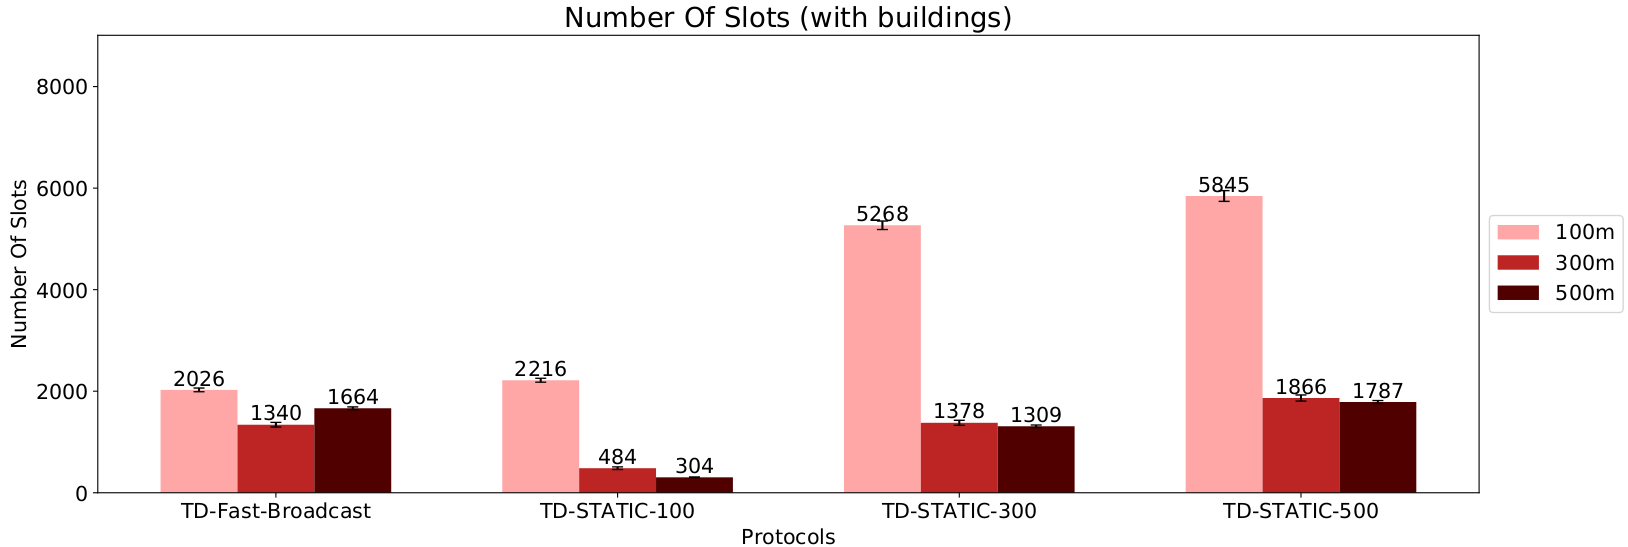
\includegraphics[width=1.0\textwidth]{immagini/td-fb-pd/td-fb/nos}	
			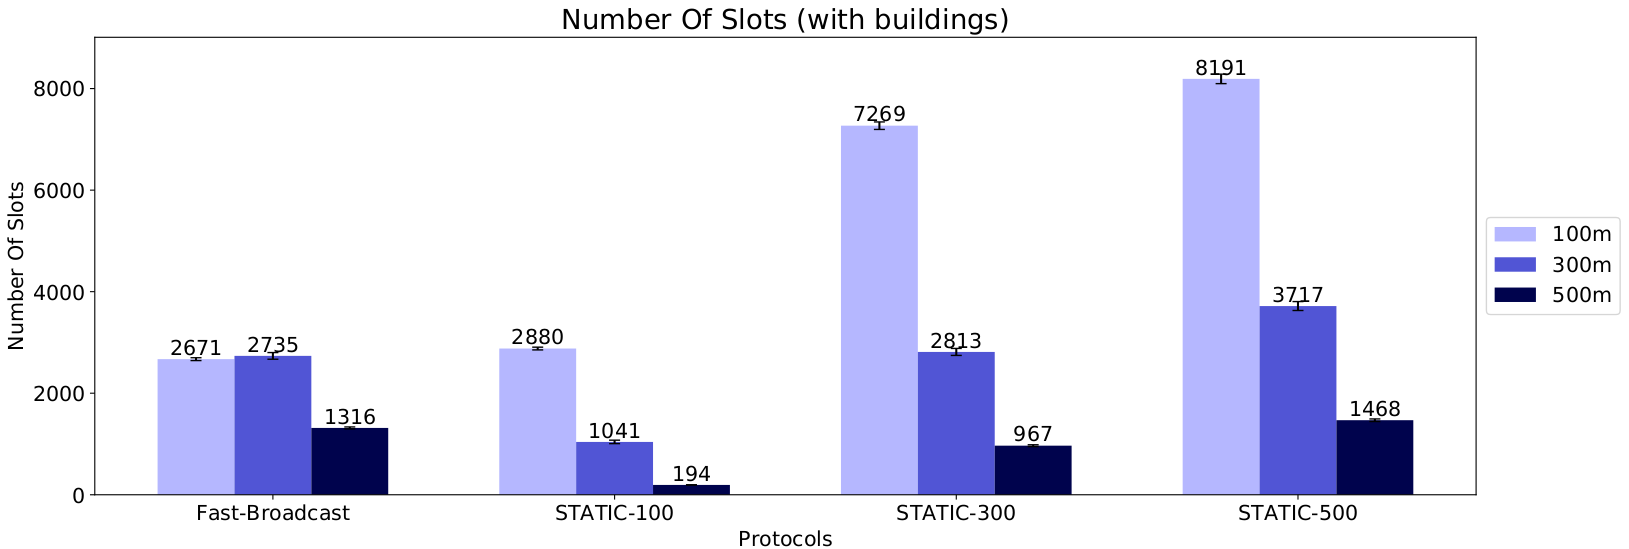
\includegraphics[width=1.0\textwidth]{immagini/td-fb-pd/fb/nos}
			\caption{\textit{NOS} for TD-Fast-Broadcast (top) and Fast-Broadcast (bottom) for Padua urban scenario}
			\label{fig:td-nos}
		\end{figure}
		
		\begin{figure}[H]
			\centering
			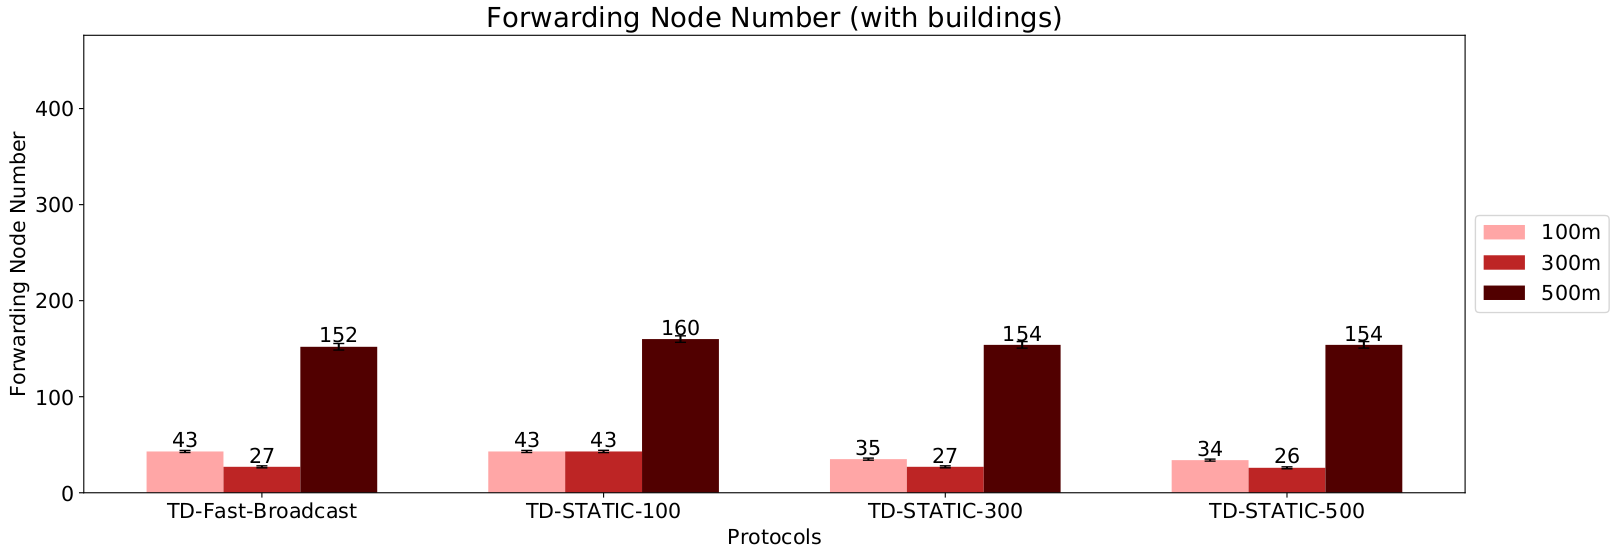
\includegraphics[width=1.0\textwidth]{immagini/td-fb-pd/td-fb/fnn}	
			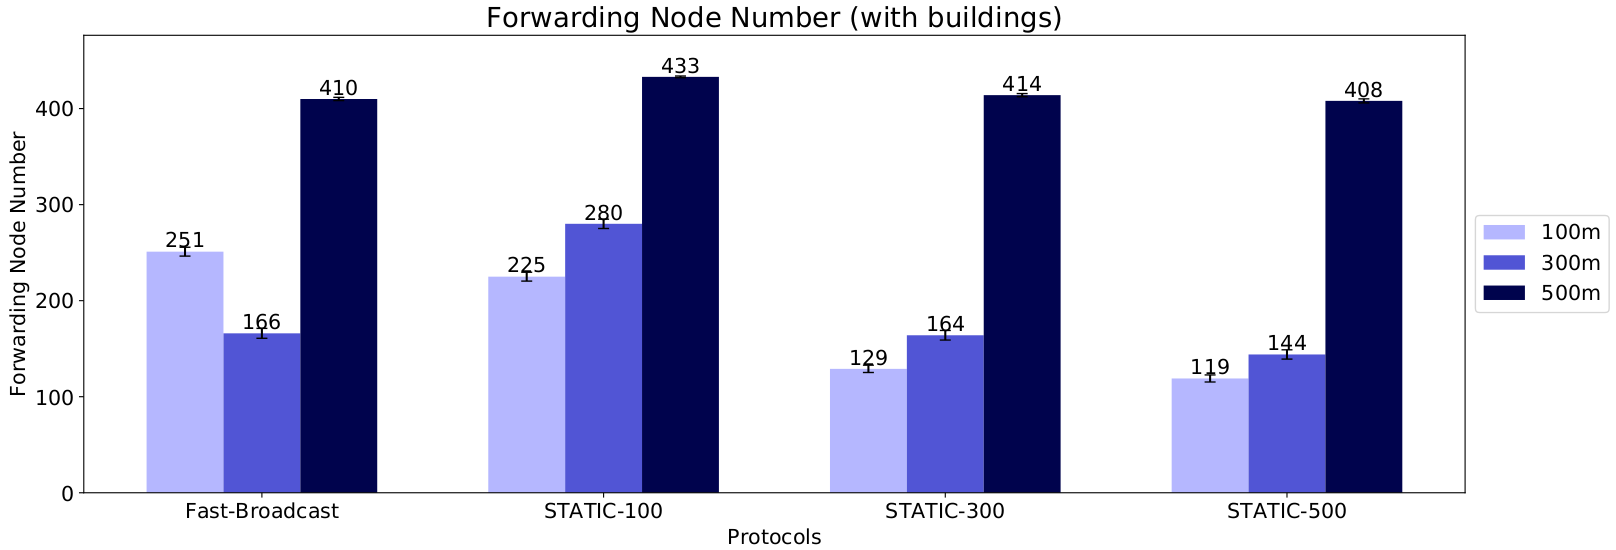
\includegraphics[width=1.0\textwidth]{immagini/td-fb-pd/fb/fnn}
			\caption{\textit{FNN} for TD-Fast-Broadcast (top) and Fast-Broadcast (bottom) for Padua urban scenario}
			\label{fig:td-fnn}
		\end{figure}

	Figure \ref{fig:td-tdr} and \ref{fig:td-tdroc} show that TD-Fast-Broadcast struggles to deliver message across the network, even with 500 meters transmission range. The results are poor especially for the lowest transmission ranges, where the achieved delivery ratios are under 10\%. The removal of the suppression based on distance improve Fast-Broadcast's delivery ratios for all three transmission range configurations. 
	
	
	Figure \ref{fig:td-noh}, \ref{fig:td-nos} and \ref{fig:td-fnn} show an increase in all three metric's value (except for \textit{NOS} with 500 meters transmission range), but it is important to remember how those metrics are calculated (Section \ref{sec:metrics}). \textit{NOS} and \textit{NOH} take into consideration the nodes on the circumference reached by the Alert Message. Fast-Broadcast reaches a greater number of nodes on the circumference, hence the metric is calculated on different sets of vehicles. Moreover, the increase in \textit{FNN} results in a greater coverage, which is a desirable property. Overall, Fast-Broadcast brings about a great increase in delivery ratios. The non pejorative effects of Fast-Broadcast on the other metrics in a scenario where TD-Fast-Broadcast delivery ratio is not poor will be analyzed in the next section.
	
	\section{Fast-Broadcast's non-pejorative effects}
		\begin{figure}[H]
			\centering	
			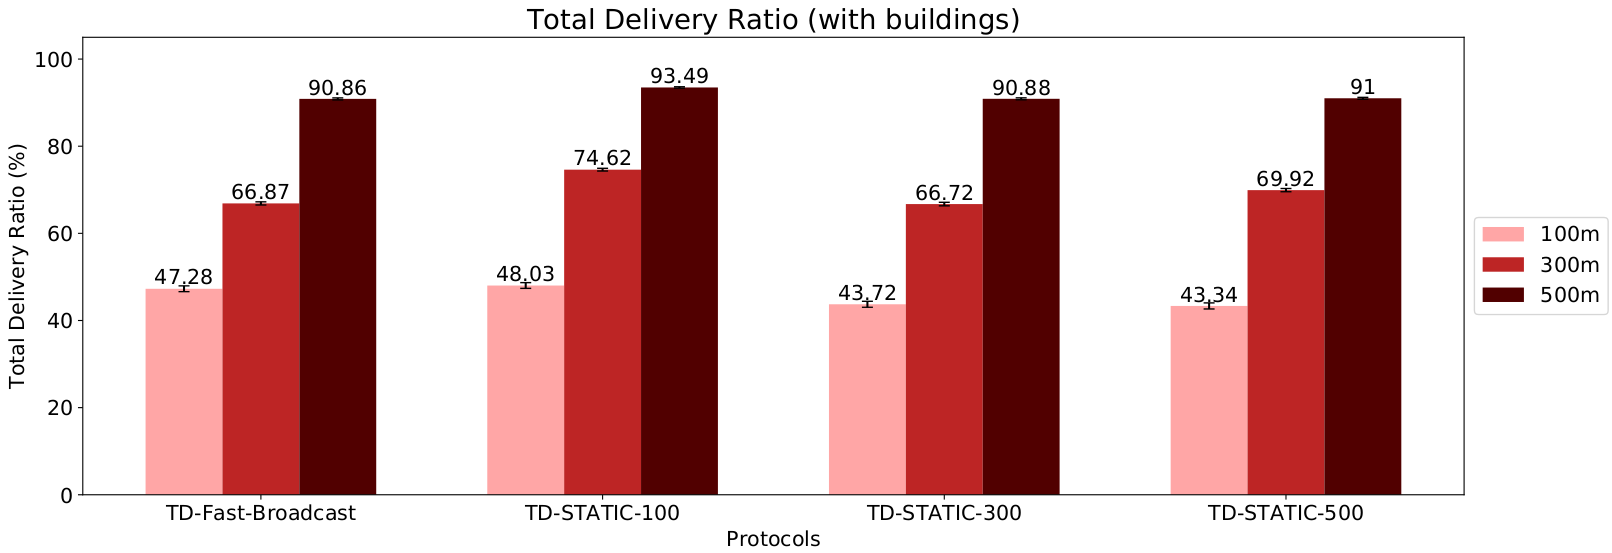
\includegraphics[width=1.0\textwidth]{immagini/td-fb-la/td-fb/tdr}
			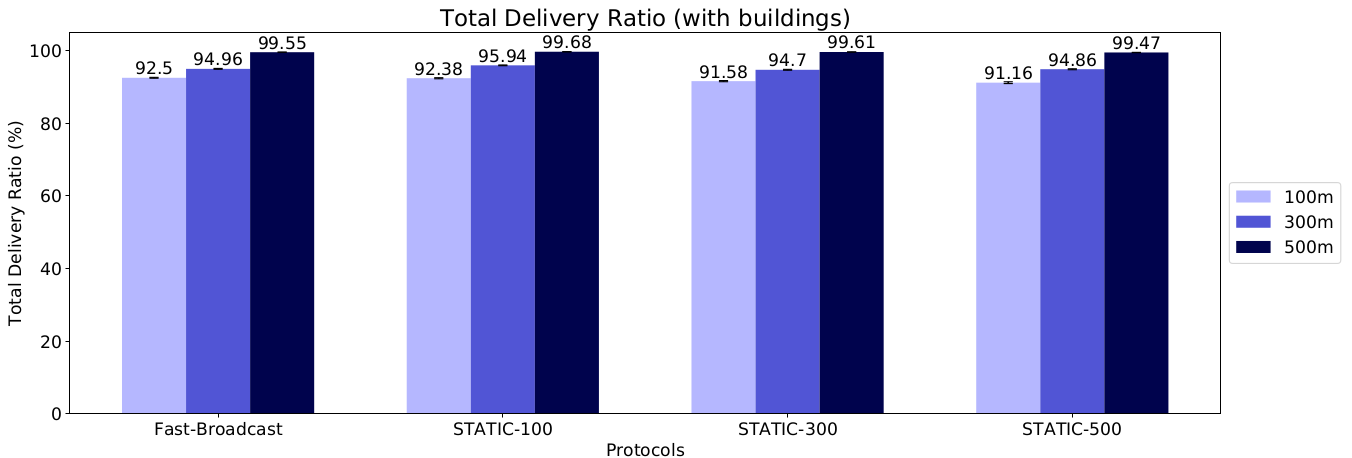
\includegraphics[width=1.0\textwidth]{immagini/td-fb-la/fb/tdr}
			\caption{\textit{TDR} for TD-Fast-Broadcast (top) and Fast-Broadcast (bottom) for Los Angeles urban scenario}
			\label{fig:la-td-tdr}
		\end{figure}
			
		\begin{figure}[H]
			\centering
			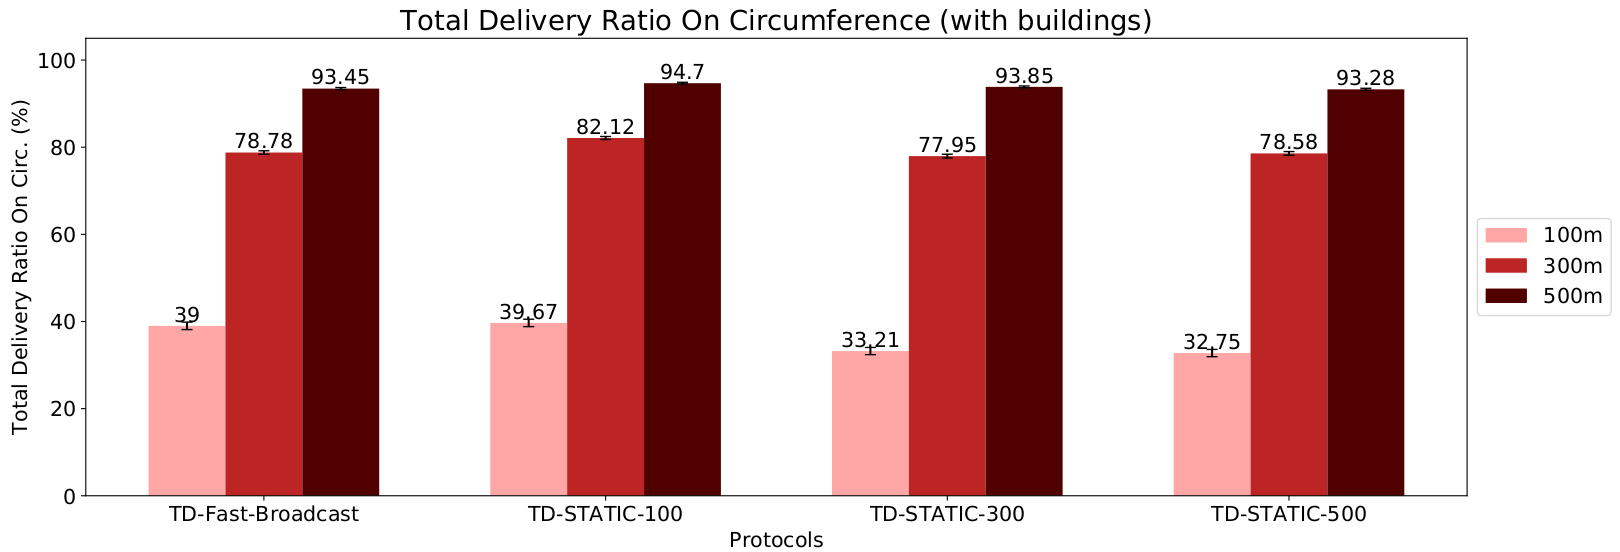
\includegraphics[width=1.0\textwidth]{immagini/td-fb-la/td-fb/tdroc}	
			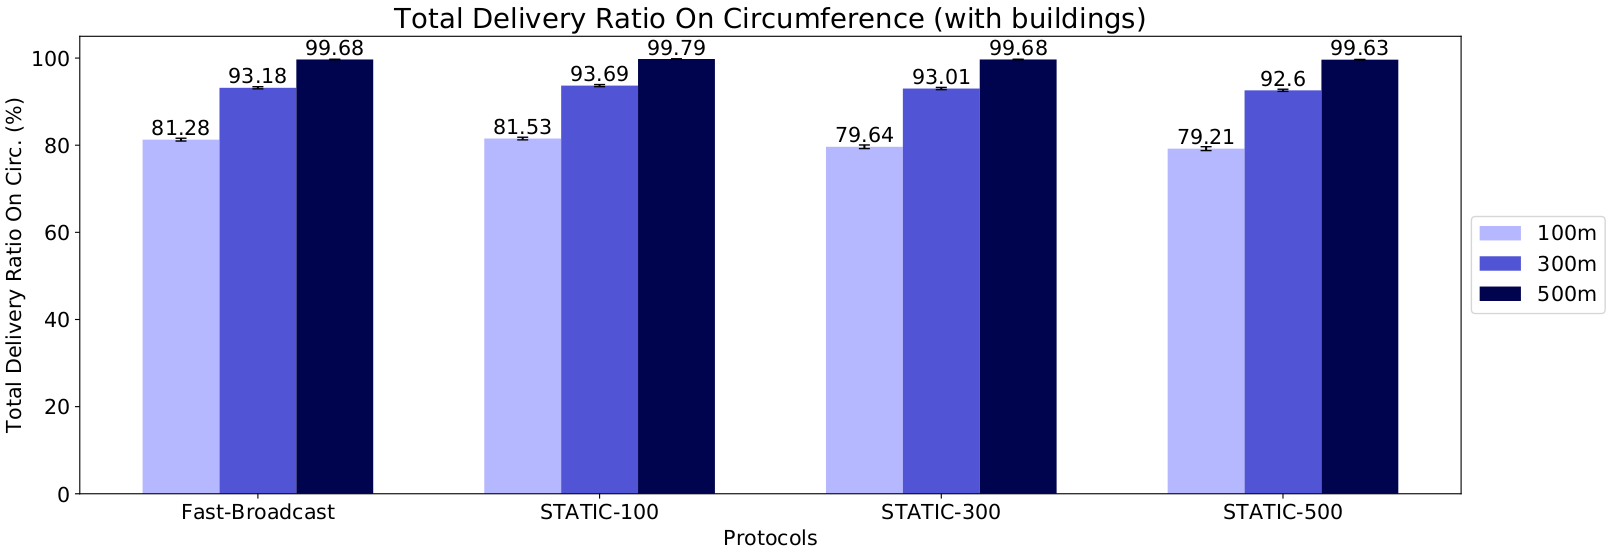
\includegraphics[width=1.0\textwidth]{immagini/td-fb-la/fb/tdroc}
			\caption{\textit{TDROC} for TD-Fast-Broadcast (top) and Fast-Broadcast (bottom) for Los Angeles urban scenario}
			\label{fig:la-td-tdroc}
		\end{figure}
				
		\begin{figure}[H]
			\centering
			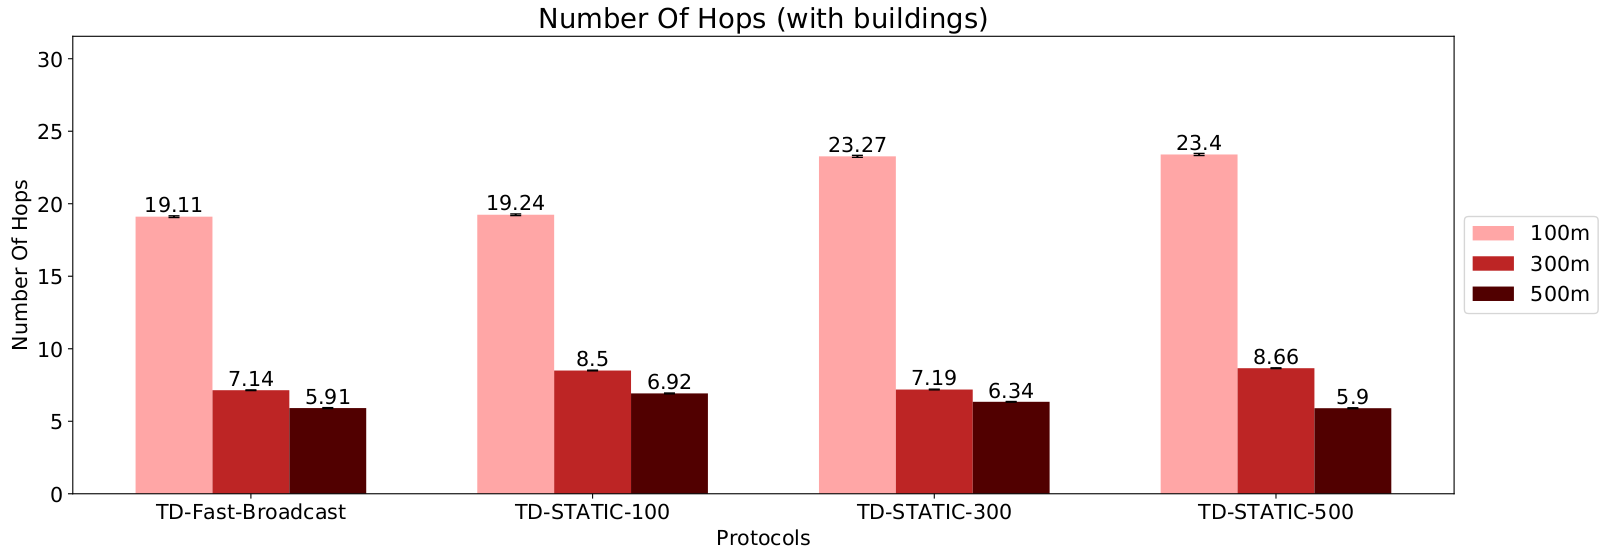
\includegraphics[width=1.0\textwidth]{immagini/td-fb-la/td-fb/noh}	
			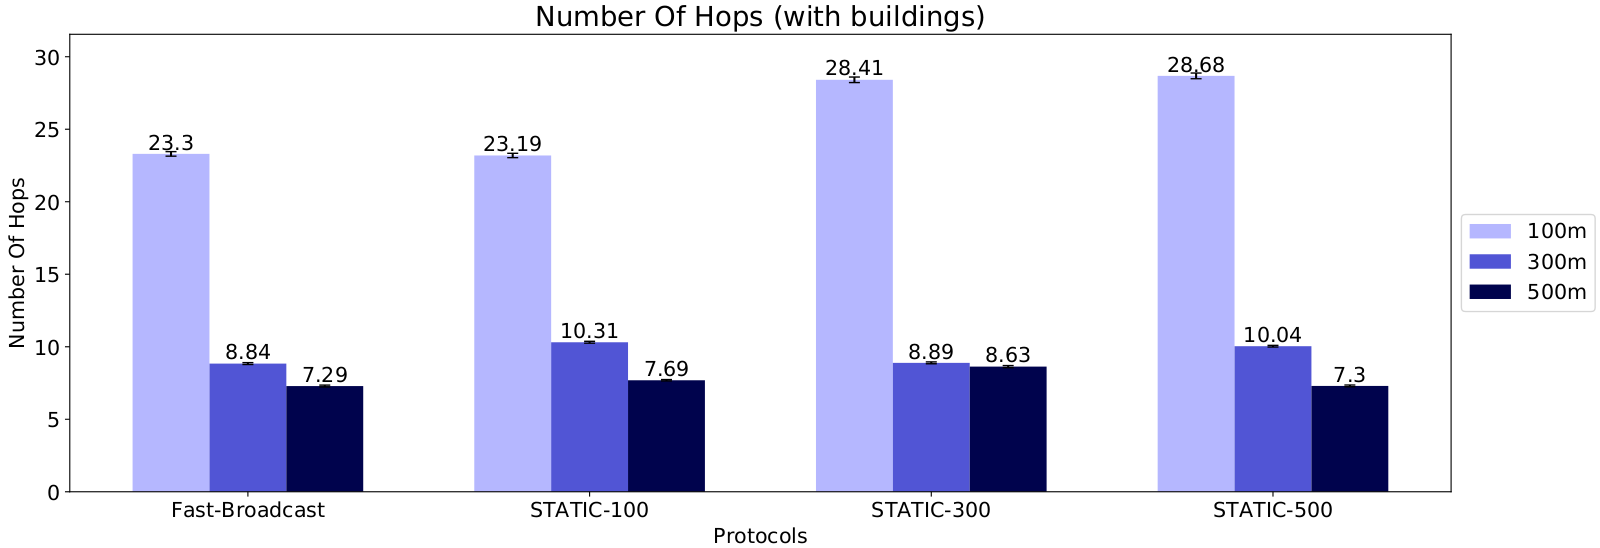
\includegraphics[width=1.0\textwidth]{immagini/td-fb-la/fb/noh}
			\caption{\textit{NOH} for TD-Fast-Broadcast (top) and Fast-Broadcast (bottom) for Los Angeles urban scenario}
			\label{fig:la-td-noh}
		\end{figure}
					
		\begin{figure}[H]
			\centering
			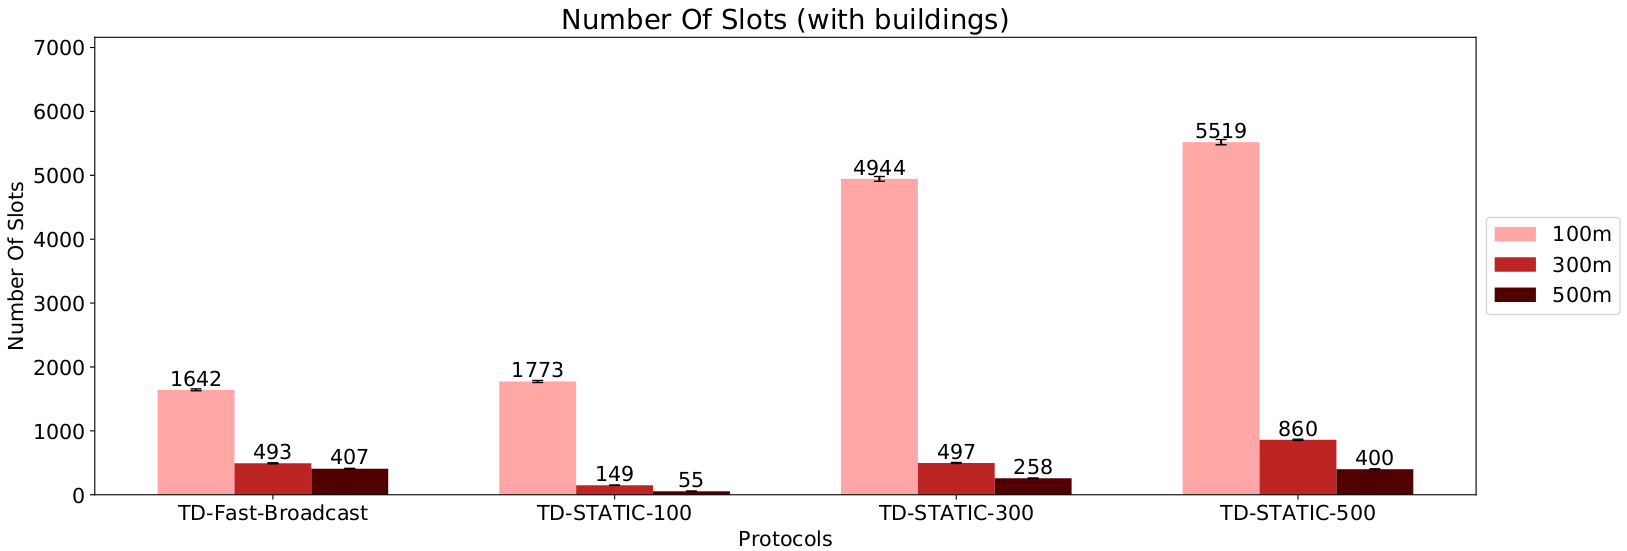
\includegraphics[width=1.0\textwidth]{immagini/td-fb-la/td-fb/nos}	
			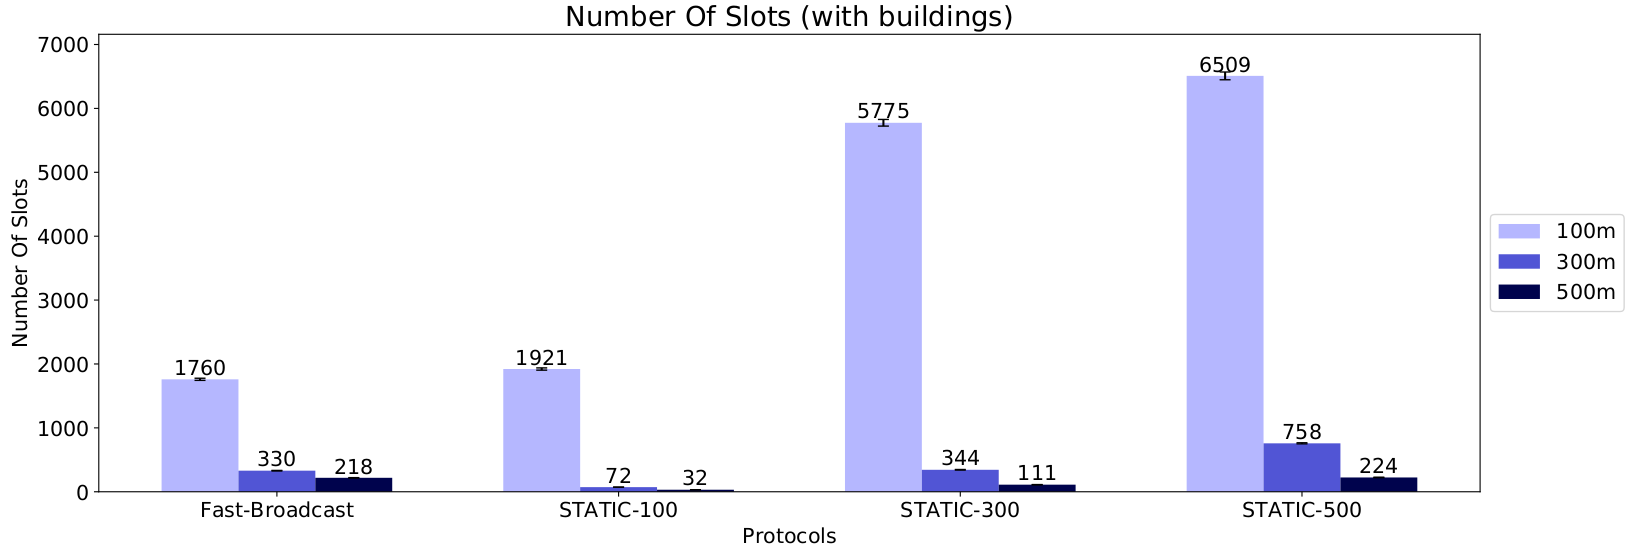
\includegraphics[width=1.0\textwidth]{immagini/td-fb-la/fb/nos}
			\caption{\textit{NOS} for TD-Fast-Broadcast (top) and Fast-Broadcast (bottom) for Los Angeles urban scenario}
			\label{fig:la-td-nos}
		\end{figure}
						
		\begin{figure}[H]
			\centering
			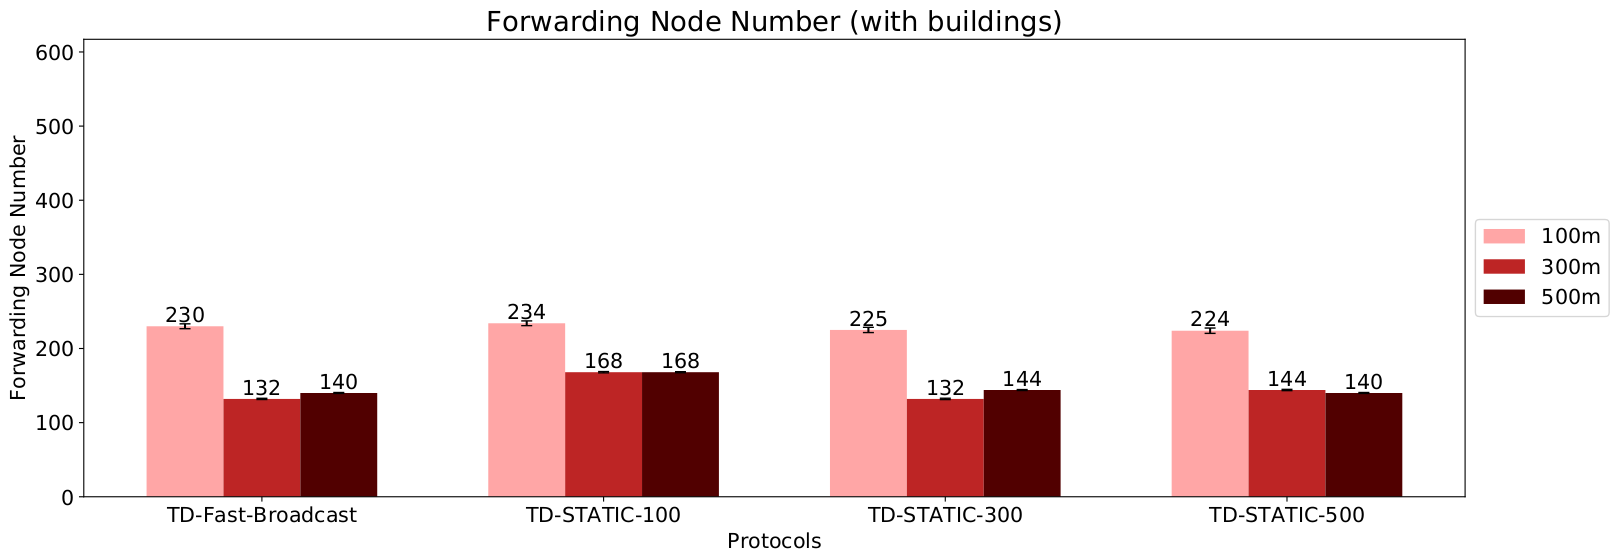
\includegraphics[width=1.0\textwidth]{immagini/td-fb-la/td-fb/fnn}	
			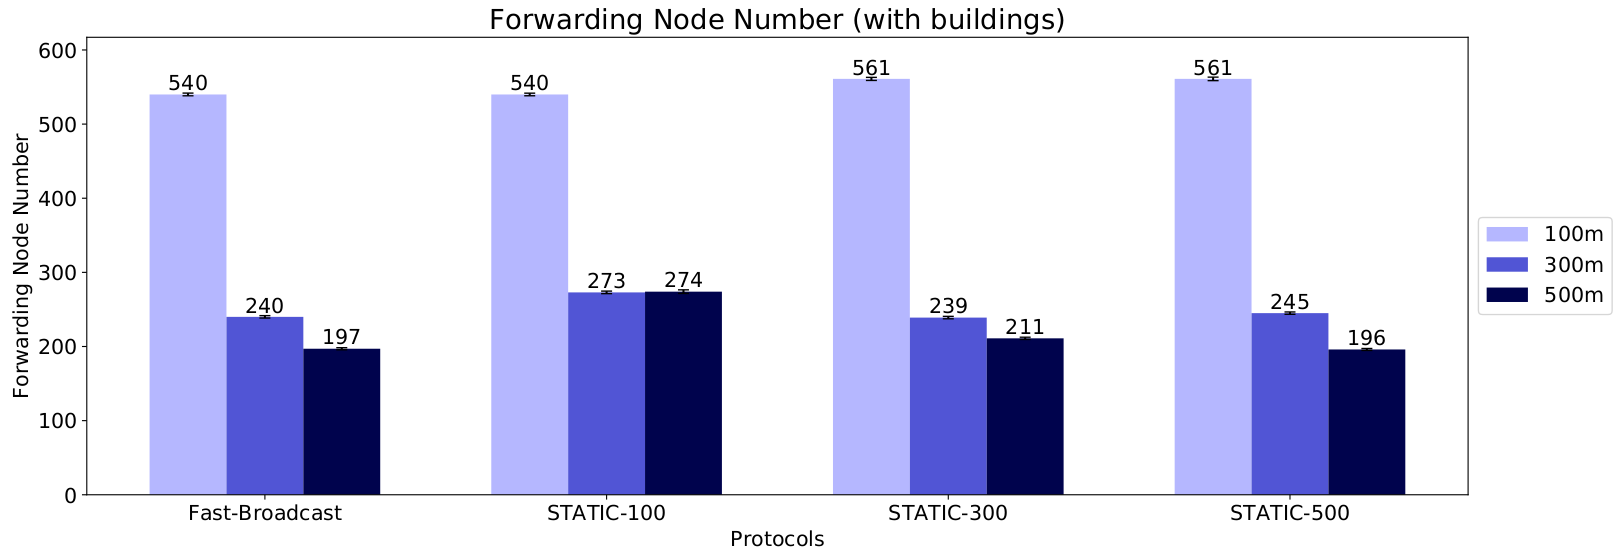
\includegraphics[width=1.0\textwidth]{immagini/td-fb-la/fb/fnn}
			\caption{\textit{FNN} for TD-Fast-Broadcast (top) and Fast-Broadcast (bottom) for Los Angeles urban scenario}
				\label{fig:la-td-fnn}
		\end{figure}
		
		The increase in delivery ratios brought about by Fast-Broadcast is visible also in this scenario. If we focus on the 500 meters transmisison range delivery ratios in Figure \ref{fig:la-td-tdr} and \ref{fig:la-td-tdroc}, the increase is not so severe (from 90.86\% to 99.55\% for \textit{TDR} and from 93.45\% to 99.68\% from \textit{TDROC}), so we will utilize this configuration to notice the non pejorative effects on the other metrics.
		\textit{NOH} (Figure \ref{fig:la-td-noh}) increases by 23.35\%, but this is coupled with a decrease in \textit{NOS} of 46.44\%. Basically, the paths taken from the source to the circumference are slightly longer in terms of hops, but the number of slots waited is a lot smaller. Overall, the decrease in \textit{NOS} outweighs the slight increase in \textit{NOH}, making Fast-Broadcast a winner under this point of view.
		
		
		Regarding \textit{FNN}, Fast-Broadcast's \textit{FNN} increases by 40.71\% compared to TD-Fast-Broadcast. Considering the slight increase in delivery ratios and the considerable increase in \textit{NOS}, such increase in the number of forwarding nodes has been deemed acceptable. 
		
		
		This observation, paired with the one exposed in the previous Section, make Fast-Broadcast a clear winner compared to TD-Fast-Broadcast. Hence, all the algorithm improvements, extensions and tests of Chapter \ref{chapter:fb} and \ref{chapter:simulations} will be based on Fast-Broadcast after the removal of the check on distances.
		
		